\documentclass{article}

\usepackage{fancyhdr}
\usepackage{extramarks}
\usepackage{amsmath}
\usepackage{amsthm}
\usepackage{amsfonts}
\usepackage{tikz}
\usepackage{multicol}
\usepackage{float}
%\usepackage[plain]{algorithm}
\usepackage[ruled,vlined]{algorithm2e}
\usepackage{algpseudocode}

\usetikzlibrary{automata,positioning}

%
% Basic Document Settings
%

\topmargin=-0.45in
\evensidemargin=0in
\oddsidemargin=0in
\textwidth=6.5in
\textheight=9.0in
\headsep=0.25in

\linespread{1.1}

\pagestyle{fancy}
\lhead{\hmwkAuthorName}
\chead{\hmwkClass\ : \hmwkTitle}
\rhead{\firstxmark}
\lfoot{\lastxmark}
\cfoot{\thepage}

\renewcommand\headrulewidth{0.4pt}
\renewcommand\footrulewidth{0.4pt}

\setlength\parindent{0pt}

%
% Create Problem Sections
%

\newcommand{\enterProblemHeader}[1]{
    \nobreak\extramarks{}{Problem \arabic{#1} continued on next page\ldots}\nobreak{}
    \nobreak\extramarks{Problem \arabic{#1} (continued)}{Problem \arabic{#1} continued on next page\ldots}\nobreak{}
}

\newcommand{\exitProblemHeader}[1]{
    \nobreak\extramarks{Problem \arabic{#1} (continued)}{Problem \arabic{#1} continued on next page\ldots}\nobreak{}
    \stepcounter{#1}
    \nobreak\extramarks{Problem \arabic{#1}}{}\nobreak{}
}

\setcounter{secnumdepth}{0}
\newcounter{partCounter}
\newcounter{homeworkProblemCounter}
\setcounter{homeworkProblemCounter}{1}
\nobreak\extramarks{Problem \arabic{homeworkProblemCounter}}{}\nobreak{}

%
% Homework Problem Environment
%
% This environment takes an optional argument. When given, it will adjust the
% problem counter. This is useful for when the problems given for your
% assignment aren't sequential. See the last 3 problems of this template for an
% example.
%
\newenvironment{homeworkProblem}[1][-1]{
    \ifnum#1>0
        \setcounter{homeworkProblemCounter}{#1}
    \fi
    \section{Problem \arabic{homeworkProblemCounter}}
    \setcounter{partCounter}{1}
    \enterProblemHeader{homeworkProblemCounter}
}{
    \exitProblemHeader{homeworkProblemCounter}
}

%
% Homework Details
%   - Title
%   - Due date
%   - Class
%   - Section/Time
%   - Instructor
%   - Author
%

\newcommand{\hmwkTitle}{Homework\ \#3}
\newcommand{\hmwkDueDate}{Dec. 2, 2019}
\newcommand{\hmwkClass}{Modern Computational Statistics}
\newcommand{\hmwkClassTime}{ }
\newcommand{\hmwkClassInstructor}{}
\newcommand{\hmwkAuthorName}{\textbf{Huang Daoji}}

%
% Title Page
%

\title{
    \vspace{2in}
    \textmd{\textbf{\hmwkClass:\ \hmwkTitle}}\\
    \normalsize\vspace{0.1in}\small{Due\ on\ \hmwkDueDate\ at 3:10pm}\\
    \vspace{0.1in}\large{\textit{\hmwkClassInstructor\ \hmwkClassTime}}
    \vspace{3in}
}

\author{\hmwkAuthorName}
\date{}

\renewcommand{\part}[1]{\textbf{\large Part \Alph{partCounter}}\stepcounter{partCounter}\\}

%
% Various Helper Commands
%

% Useful for algorithms
\newcommand{\alg}[1]{\textsc{\bfseries \footnotesize #1}}

% For derivatives
\newcommand{\deriv}[1]{\frac{\mathrm{d}}{\mathrm{d}x} (#1)}

% For partial derivatives
\newcommand{\pderiv}[2]{\frac{\partial}{\partial #1} (#2)}

% Integral dx
\newcommand{\dx}{\mathrm{d}x}

% Alias for the Solution section header
\newcommand{\solution}{\textbf{\large Solution}}

% Probability commands: Expectation, Variance, Covariance, Bias
\newcommand{\E}{\mathrm{E}}
\newcommand{\Var}{\mathrm{Var}}
\newcommand{\Cov}{\mathrm{Cov}}
\newcommand{\Bias}{\mathrm{Bias}}

\begin{document}

%\maketitle

\pagebreak

\begin{homeworkProblem}

\textbf{(1)}

For each datapoint $y_i$, we introduce a latent variable $z_i$, which indicates the normal distribution $y_i$ is from, $i.e.$ $z_i = 0 \iff y_i$ is from $N(\mu_1, \sigma_1^2)$ and vice versa. The EM algorithm is derived below. \\

In E-step, we first derive $p(z_n = k | x_n, \theta)$ using Bayesian formula where $\theta$ denotes $\mu_i, \sigma^2_i, w$.

\begin{equation}
    \begin{aligned}
        p(z_n = k | y_n, \theta) &= \frac{p(z_n = k, y_i | \theta)}{\sum_k p(z_n = k, y_i | \theta)} \\
        &= \frac{w_k N(y_i | \mu_k, \sigma^2_k)}{\sum_k w_k N(y_i | \mu_k, \sigma^2_k)} \\
        &= \gamma_{n, k}
    \end{aligned}
\end{equation}

where $\gamma_{n, k}$ can be seen as a soft label of latent variable $z_n$. The log likelihood function is then

\begin{equation}
    \begin{aligned}
        l(\theta) &= \sum_n \sum_k p(z_k | x_n, \theta) \log p(z_k, x_n | \theta) \\
        &= \sum_n \sum_k \gamma_{n, k} (\log w_k - \frac{1}{2} 2\pi - \frac{1}{2}\log \sigma_k^2) - \frac{(y_n - \mu_k)^2}{2\sigma_k^2}
    \end{aligned}
\end{equation}

In M-step, we take the derivative of $l(\theta)$, and set it to zero w.r.t. $w_k, \mu_k$ and $\sigma_k$. \\

a) max $l(\theta)$ w.r.t. $w_k$, using Lagrange multiplier since $\sum w_k = 1$

\begin{equation}
    \begin{aligned}
        \sum_n \sum_k \gamma_{n, k} \frac{1}{w_k} - \lambda &= 0, \ \ \ \forall k \\
        w_k &\propto \sum_n \gamma_{n, k} \\
        w_k &= \frac{\sum_n \gamma_{n, k}}{\sum_k \sum_n \gamma_{n, k}}
    \end{aligned}
\end{equation}

b) max $l(\theta)$ w.r.t. $\mu_k$

\begin{equation}
    \begin{aligned}
        \sum_n \gamma_{n, k} \frac{(y_n - \mu_k)}{\sigma_{k}^{2}} &= 0 \\
        \mu_k &= \frac{\sum_{n} \gamma_{n, k} y_n}{\sum_n \gamma_{n, k}}
    \end{aligned}
\end{equation}

c) max $l(\theta)$ w.r.t. $\sigma^2_k$

\begin{equation}
    \begin{aligned}
        \sum_{n} \gamma_{n, k} (-\frac{1}{2\sigma_k^2} + \frac{(y_n - \mu_k)^2}{2(\sigma_{k}^2)^2}) &= 0 \\
        \sigma_k^2 &= \frac{\sum_n \gamma_{n, k}(y_n - \mu_k)^2}{\sum_n \gamma_{n, k}}
    \end{aligned}
\end{equation}

The EM algorithm is shown below \\

\begin{algorithm}[H]
    \SetAlgoLined
    \caption{EM for GMM}
    \KwResult{$\mu, \sigma^2, w$}
    \Begin{
        initialize $\mu, \sigma^2, w$ \\
        \While{not converge}{
            calculate $\gamma_{n, k}$ \\
            update $\mu, \sigma^2, w$
        }
    }
\end{algorithm}

\textbf{(2)}

EM algorithm does not always converge on this dataset. In my implementation, four modes are found.

\begin{figure}[!htb]
\minipage{0.49\textwidth}
  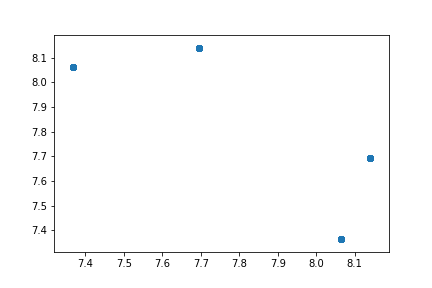
\includegraphics[width=\linewidth]{./mu_mode.png}
  \caption{results of $\mu$}\label{fig:awesome_image1}
\endminipage\hfill
\minipage{0.49\textwidth}%
  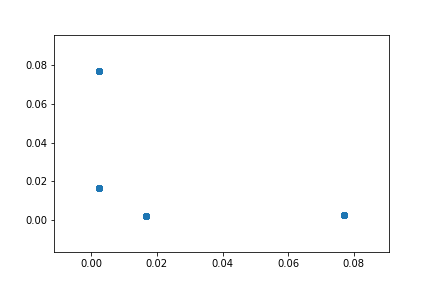
\includegraphics[width=\linewidth]{./sigma_mode.png}
  \caption{results of $\sigma^2$}\label{fig:awesome_image3}
\endminipage
\end{figure}

\end{homeworkProblem}

\begin{homeworkProblem}

\textbf{(1)}

The likelihood function for $\theta$ is

\begin{equation}
    L(\theta) = \prod_n e^{-(x_n \theta + r_n)} \frac{(x_n \theta + r_n)^{y_n}}{y_n!}
\end{equation}

\textbf{(2)}

Similar to the E-step in Problem1, we first calculate $E(z_{j1} | x_{j}, \theta)$. Notice that $z_{j1} | y_j \sim Binominal(y_j, \frac{x_j \theta}{x_{j} \theta + r_j})$. No need to calculate $E(z_{j2} | x_{j}, \theta)$ since it's irrelevant to $\theta$ in log likelihood function.

\begin{equation}
    E(z_{j1} | x_{j}, \theta) = y_j \frac{x_j \theta}{x_{j} \theta + r_j}
\end{equation}

In M-step, we derive its log likelihood function first

\begin{equation}
    \begin{aligned}
        l(\theta) &= \sum_j -x_k + z_{j1} \log x_j \theta - \log z_{j1}! - r_j + z_{j2} \log r_j - \log z_{j2}! \\
        \frac{d l(\theta)}{d\theta} &= \sum_j -x_j + z_{j1} \frac{1}{\theta}
    \end{aligned}
\end{equation}

Substitute $z_{j1}$ by $E(z_{j1} | x_{j}, \theta)$(since $\theta$ is irrelevant to $z_{j1}$) and set the derivative to zero, we have

\begin{equation}
    \theta' = \frac{\theta}{\sum_j x_j} \sum_j \frac{y_j x_j}{x_j \theta + r_j}
\end{equation}

which can be seen as a fix point iteration of true likelihood function.

\begin{algorithm}[H]
    \SetAlgoLined
    \caption{EM for sum of Poission}
    \KwResult{$\theta$}
    \Begin{
        initialize $\theta$ \\
        \While{not converge}{
            calculate $E(z_{j1} | x_{j}, \theta)$ \\
            update $\theta$
        }
    }
\end{algorithm}

\textbf{(3)}

The MLE is 5.606063396561341, which yields 1.78e-15 in true likelihood function.

\textbf{(4)}

By taking second derivative of log likelihood function in \textbf{(1)}, we have

\begin{equation}
    \begin{aligned}
        -\frac{\partial^2 l(\theta)}{\partial \theta^2} &= \sum_n y_n \frac{x_n^2}{(x_n \theta + r_n)^2} \\
        &= 2.423
    \end{aligned}
\end{equation}

, and the complete information being

\begin{equation}
    \begin{aligned}
        -\frac{\partial^2 q(\theta)}{\partial \theta^2} &= \sum_n y_n \frac{x_n}{(x_n \theta + r_n) \theta} \\
        &= 2.588
    \end{aligned}
\end{equation}

, so the fraction of missing information is 0.064

\end{homeworkProblem}


\begin{homeworkProblem}

\textbf{(1)}

\begin{equation}
    \begin{aligned}
        l(\pi) &= 100\log \pi_{11} + 50 \log \pi_{12} + 75 \log \pi_{21} + 75 \log \pi_{22} \\
        &+ 28 \log (\pi_{11} + \pi_{12}) + 60 \log (\pi_{21} + \pi_{22}) + 30 \log (\pi_{11} + \pi_{21}) + 60 \log (\pi_{12} + \pi_{22})
    \end{aligned}
\end{equation}

The assumption under such a log likelihood includes
\begin{itemize}
    \item outcomes of $Y_1, Y_2$ and that whether one of the outcomes is missing are independent, $i.e.$ the fact that one of the outcomes is missing does not effect the prob. of that outcome
\end{itemize}

\textbf{(2)}

We derive the likelihood funtion for all data first

\begin{equation}
    L(\pi) = \prod_n \pi_{11}^{y_{n1} = 1, y_{n2} = 1}
    \pi_{12}^{y_{n1} = 1, y_{n2} = 2}
    \pi_{21}^{y_{n1} = 2, y_{n2} = 1}
    \pi_{22}^{y_{n1} = 2, y_{n2} = 2}
\end{equation}

E-step: For the observed 300 cases, all $y_{n1}, y_{n2}$ are observed thus fixed, while for missing data, one of them need to be estimated, e.g. for the 28 datapoints with $Y_1$ missing, the estimation is simply from Bayesian formula

\begin{equation}
    p(y_{n1} = 1, y_{n2} = 1) = \frac{\pi_{11}}{\pi_{11} + \pi_{12}},\
    p(y_{n1} = 1, y_{n2} = 2) = \frac{\pi_{12}}{\pi_{11} + \pi_{12}}
\end{equation}

We do this for all missing data.

In M-step, we take the derivative of log likelihood function and set it to zero w.r.t. $\pi_{ij}$

\begin{equation}
    \begin{aligned}
        \sum_n p(y_{n1} = i, y_{n2} = j) / \pi_{ij} - \lambda &= 0 \\
        \pi_{ij} &\propto \sum_n p(y_{n1} = i, y_{n2} = j) \\
        \pi_{ij} &= \sum_n p(y_{n1} = i, y_{n2} = j) / \sum_{i, j}\sum_n p(y_{n1} = i, y_{n2} = j)
    \end{aligned}
\end{equation}

\textbf{(3)}

The MLE of $\pi$ from EM algorithm is [0.27912927 0.17190756 0.24112718 0.30783599]

\textbf{(4)}

The odds ratio from complete data is 100 * 75 / (75 * 50) = 2.0, while that from MLE is 2.07, not equal.

\end{homeworkProblem}

\end{document}
